
%(BEGIN_QUESTION)
% Copyright 2012, Tony R. Kuphaldt, released under the Creative Commons Attribution License (v 1.0)
% This means you may do almost anything with this work of mine, so long as you give me proper credit

Electrically-powered air compressors are commonly used in many different industries for supplying clean, dry compressed air to machines, instrument systems, and pneumatic tools.  A simple compressor system consists of a compressor which works much like a bicycle tire pump (drawing in air, then compressing it using pistons), an electric motor to turn the compressor mechanism via a V-belt, a ``receiver tank'' to receive the compressed air discharged by the compressor mechanism, and some miscellaneous components installed to control the pressure of the compressed air in the receiver tank and drain any condensed water vapor that enters the receiver:

$$\includegraphics[width=15.5cm]{i02540x01.eps}$$

Electromechanical relay circuitry located inside the electrical enclosure decides when to turn the compressor motor on and off based on the statuses of the high- and low-pressure control switches (PSH = high pressure switch ; PSL = low pressure switch).  

\vskip 10pt

Your task is two-fold.  First, you must figure out how to wire a new low-low pressure alarm switch (PSLL, shown on the left-hand end of the receiver) so that an alarm buzzer will activate if ever the compressed air pressure falls too low.  A newly-installed hand switch located on the front panel of the electrical enclosure must be wired with this PSLL switch in such a way that the buzzer cannot energize if the hand switch is in the ``alarm disable'' position.  Second, you must figure out how to wire a new high-level switch (LSH, shown on the ``boot'' of the receiver tank) so that the condensate drain valve will energize automatically to open up and drain water out of the receiver boot when the level gets too high, and then automatically shut again when the water in the boot drops down to an acceptable level.

\vskip 10pt

\filbreak

The following schematic diagram shows the basic motor control circuit for this air compressor, with the new switches, buzzer, and drain valve shown unwired:

$$\includegraphics[width=15.5cm]{i02540x02.eps}$$

Complete this control circuit by sketching connecting wires between the new switches, buzzer, and drain valve solenoid.  Remember that the way all switches are drawn in schematic diagrams is in their ``normal'' states as defined by the manufacturer: the {\it state of minimum stimulus} (when the switch is un-actuated).  For pressure switches, this ``normal'' state occurs during a low pressure condition; for liquid level switches, this ``normal'' state occurs during a low-level (dry) condition.  Note that each of the new process switches has SPDT contacts, allowing you to wire each one as normally-open (NO) or as normally-closed (NC) as you see fit.


\underbar{file i02540}
%(END_QUESTION)





%(BEGIN_ANSWER)

\noindent
{\bf Partial answer:} (this is just one possible solution to the wiring of the pressure switch):

$$\includegraphics[width=15.5cm]{i02540x03.eps}$$

%(END_ANSWER)





%(BEGIN_NOTES)

$$\includegraphics[width=15.5cm]{i02540x04.eps}$$






\filbreak

\filbreak \vskip 20pt \vbox{\hrule \hbox{\strut \vrule{} {\bf Virtual Troubleshooting} \vrule} \hrule}

$$\includegraphics[width=15.5cm]{i02540x05.eps}$$

\noindent
{\bf Predicting the effect of a given fault:} present each of the following faults to the students, one at a time, having them comment on all the effects each fault would produce.

\begin{itemize}
\item{} Fuse F1 blows
\item{} Fuse F2 blows
\item{} Fuse F3 blows
\item{} (Any) OL ``heater'' fails open
\item{} Wire H2-H3 fails open
\item{} PSH fails open
\item{} PSL fails open
\item{} PSLL fails open
\item{} LSH fails open
\item{} M1 seal-in contact fails open
\item{} M1 seal-in contact fails shorted
\item{} M1 coil fails open
\item{} M1 coil fails shorted
\end{itemize}


\vskip 10pt


\noindent
{\bf Identifying possible/impossible faults:} suppose the compressor motor refuses to start with the Run/Stop switch in the ``Run'' position.  Using a voltmeter, you measure 120VAC between points D and L.  Present these symptoms to the students and then have them determine whether or not a series of suggested faults could account for all the symptoms, explaining {\it why} or {\it why not} for each proposed fault:

\begin{itemize}
\item{} Fuse F1 blows
\item{} Fuse F2 blows
\item{} Fuse F3 blows
\item{} (Any) OL ``heater'' fails open
\item{} Wire H2-H3 fails open
\item{} Wire E-H fails open
\item{} PSH fails open 
\item{} PSL fails open
\item{} PSLL fails open
\item{} LSH fails open
\item{} M1 seal-in contact fails open
\item{} M1 seal-in contact fails shorted
\item{} M1 coil fails open
\item{} M1 coil fails shorted
\end{itemize}


\vskip 10pt


\noindent
{\bf Determining the utility of given diagnostic tests:} imagine the ??? fails ??? in this system (but don't tell this to students!).  Present the operator's observation(s) to the students, have them consider possible faults and diagnostic strategies, and then propose the following diagnostic tests one by one.  Have students rate the value of each test, determining whether or not each test would give us useful information (i.e. tell us something we don't already know).  Also have students describe what re

\begin{itemize}
\item{} {\it }
\item{}  -- {\bf Yes/No}
\item{}  -- {\bf Yes/No}
\end{itemize}


\vskip 10pt


\noindent
{\bf Diagnosing a fault based on given symptoms:} imagine the ??? fails ??? in this system (but don't tell this to students!).  Present the operator's observation(s) to the students, have them consider possible faults and diagnostic strategies, and then tell them the results of tests they propose based on the following symptoms, until they have properly identified the nature and location of the fault:

\begin{itemize}
\item{} {\it }
\item{} 
\item{} 
\end{itemize}


%INDEX% Measurement, pressure: switch

%(END_NOTES)


